\documentclass[12px]{article}
\setlength{\parindent}{4em}
\usepackage[margin=2cm]{geometry}
\usepackage{graphicx}
\usepackage{amsmath}
\usepackage{amssymb}
\usepackage{enumerate}
\usepackage{pifont}
\usepackage{multicol}
\usepackage{booktabs}
\usepackage{array}
\linespread{1.5}

\begin{document}
%Title%
\begin{center}
    \huge\textbf {Section 1. Basic Functions and Models}
\end{center}
\large\begin{enumerate}
    %Mathematic Language%
    \item Mathematic Language
    \begin{table}[!ht]
        \centering
        \begin{tabular}[t]{p{5cm}<{\centering}p{5cm}<{\centering}}\toprule
            \textbf{Symbol} & \textbf{Meaning} \\ \midrule
            $\forall$ & For all \\ 
            $\exists$ & There exist \\ 
            $s.t.$ & Such that \\ 
            $\in$ & Belong to \\ 
            $Q.E.D$& Proof complete \\
            \bottomrule
         \end{tabular}
    \end{table}

    %Genres of Functions%
    \item Genres of Functions
    \begin{multicols}{2}
        \begin{enumerate}[(1)]    
            \item Linear Funtions
            \item Polynomials
            \item Power Functions
            \item Root Functions
            \item Reciprocal Functions
            \item Rational Functions
            \item Algebraic Functions
            \item Trigonometric Functions
            \item Exponential Functions
            \item Logarithmic Functions
            \item Inverse Functions
        \end{enumerate}
    \end{multicols}

    %The Number e%
    \item The Number e\\
    Some of the functions in calculus will be greatly simplified if we choose the base "e" of an exponential function ($y=e^x$)\ so that the the slope of tangent line at (0,1) is exactly 1. \\
    \\
    \begin{center}
        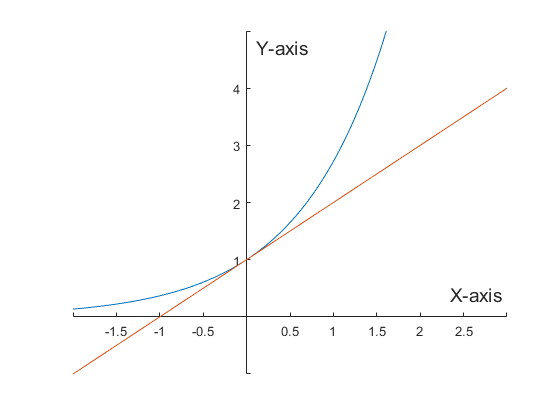
\includegraphics[width=8cm]{euler number graph.png}\\
    \end{center}

    %Inverse Functions%
    \item Inverse Functions\\
    \hspace*{2em} We can see from the graph below, as we input the variables in part A into a function, let’s say $f(x)$, we then get the corresponding answer, as shown in part B. Reversely, we can get the original values in part A by inputting the answers we just got in part B into the other function, this function is then termed $f^{-1}(x)$.\\
    \hspace*{2em} When solving these functions, the procedures are given below:
    \begin{enumerate}[(1).]
        \item Let $f^{-1}(x)=y$, then\ $f(y)=x$.
        \item Find the domain and range of the function.
        \item Finalize
    \end{enumerate}
    \begin{center}
        \includegraphics*[width=12cm]{Projection of the function.png}
    \end{center}

    %Inverse Trigonometric Function%
    \item Inverse Trigonometric Functions\\
    \hspace*{2em} When solving inverse trigonometric functions, remember to note that since trigonometric functions are not one-to-one functions, therefore, we must restrict their domains to make sure that the inverse functions we get later will not an one-to-many functions.
    \begin{equation}
        \begin{aligned}
<<<<<<< HEAD
            x=\sin^{-1}y\Leftrightarrow \sin x=y\qquad &Domain: \underline{\qquad}\leq x\leq \underline{\qquad}\quad Range: \underline{\qquad}\leq y\leq \underline{\qquad} \nonumber \\
            x=\cos^{-1}y\Leftrightarrow \cos x=y\qquad &Domain: \underline{\qquad}\leq x\leq\underline{\qquad}\ \ \; Range: \underline{\qquad}\leq y\leq \underline{\qquad} \nonumber \\
            x=\tan^{-1}y\Leftrightarrow \tan x=y\qquad  &Domain: \underline{\qquad\qquad} \qquad\qquad\, Range: \underline{\qquad}\leq y\leq \underline{\qquad} \nonumber \\
=======
            x=\sin^{-1}y\Leftrightarrow \sin x=y\qquad &Domain: \frac{-\pi}{2}\leq x\leq \frac{\pi}{2}\quad Range: -1\leq y\leq 1 \nonumber \\
            x=\cos^{-1}y\Leftrightarrow \cos x=y\qquad &Domain: 0\leq x\leq\pi\qquad\; Range: -1\leq y\leq 1 \nonumber \\
            x=\tan^{-1}y\Leftrightarrow \tan x=y\qquad  &Domain: x\in \mathbb{R} \qquad\qquad Range: \frac{-\pi}{2}\leq y\leq \frac{\pi}{2} \nonumber \\
>>>>>>> 52e6ccf1c6b4ba3cee5d6bd1d8f3bf5f5b557252
        \end{aligned}
    \end{equation}
    To better understand the concept of these functions, let’s look at some examples.
    \begin{enumerate}[(1).]
        \item Example 1\\
        Find the value of $\ \cos\;(\;2\sin^{-1}\;(\frac{3}{5}))$\\
        \\
        \\
        \\
        \item Example 2\\
        Simplify the expression $\ \cos\;(\;\sin\;(\;\tan^{-1}\;(\frac{\pi}{7})))$\\
        \\
        \\
        \\
    \end{enumerate}

    %Application of Calculus%
    \item Application of Calculus
    \begin{enumerate}[(1).]
        \item Physics\\
        \hspace*{2em}Assume you drop a ball from the window of TR-615, we’ve learned how to calculate the displacement and velocity of the ball in ideal condition in high school physics. However, in reality, we have to consider external force such as drag, in this case, we have to use Calculus.
        \item Engineering
        \begin{enumerate}[i.]
            \item Automatic Control\\
            \hspace*{2em}Suppose there’s a ball on the corner of a rectangle plate, and you’re asked to balance the ball on the center of the plate, it might not be difficult to balance it.\\ 
            \hspace*{2em}However, if you want to control a machine to balance the ball, you can use some controlling methods. For example, you can use PID control to complete it. Before doing so, you have to learn calculus :)))

            \item Diffusion\\
            \hspace*{2em} While manufacturing semiconductors, sometimes we have to dope impurities into the wafer, when doing so, we have to calculate the relationship between impurities concentration and time by Fick’s Second Law, to achieve this calculation, calculus is necessary:))))
        \end{enumerate}
        \item Computer Science\\
        \hspace*{2em} I believe everyone had used Chat-GPT, which is a Large Language Model(LLM). Have you ever thought how GPT-4 model was trained? The training of a Deep-Learning-Model has involved a large number of Functions, Statistics and more advanced mathematic concepts, and Calculus is the basis of everything.
        
    \end{enumerate}
\end{enumerate}
\end{document}